% LTeX: language=it

\chapter{Architettura del compilatore}
\label{chap:architettura-del-compilatore}

\begin{figure}[H]
	\centering
	\scalebox{0.8}{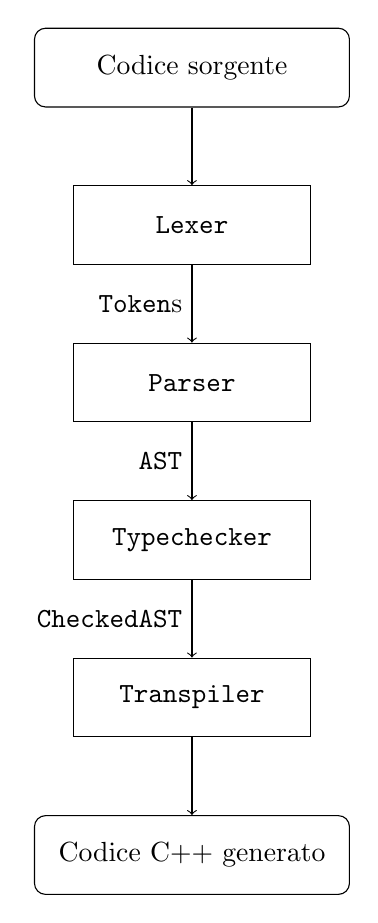
\begin{tikzpicture}[node distance=2cm]
		\node (source) [draw, rectangle, text centered, minimum width=4cm, minimum height=1cm, rounded corners] {Codice sorgente};
		\node (lexer) [below of=source, draw, rectangle, text centered, minimum width=3cm, minimum height=1cm] {\texttt{Lexer}};
		\node (parser) [below of=lexer, draw, rectangle, text centered, minimum width=3cm, minimum height=1cm] {\texttt{Parser}};
		\node (typechecker) [below of=parser, draw, rectangle, text centered, minimum width=3cm, minimum height=1cm] {\texttt{Typechecker}};
		\node (transpiler) [below of=typechecker, draw, rectangle, text centered, minimum width=3cm, minimum height=1cm] {\texttt{Transpiler}};
		\node (output) [below of=transpiler, draw, rectangle, text centered, minimum width=4cm, minimum height=1cm, rounded corners] {Codice C++ generato};

		\draw [->] (source) -- (lexer);
		\draw [->] (lexer) to node[left] {\texttt{Token}s} (parser);
		\draw [->] (parser) to node[left] {\texttt{AST}} (typechecker);
		\draw [->] (typechecker) to node[left] {\texttt{CheckedAST}} (transpiler);
		\draw [->] (transpiler) -- (output);
	\end{tikzpicture}}
	\caption{Moduli del processo di compilazione}
	\label{fig:moduli-compilatore}
\end{figure}

Nel seguente capitolo si descrive l'architettura del compilatore BugginOut, affrontando i moduli che lo compongono e le fasi del compilatore che realizzano. Nella figura sopra si pu\`o osservare l'architettura ad alto livello del compilatore che \`e costituito da quattro moduli principali:
\begin{itemize}
	\item \texttt{Lexer}: realizza l'analisi lessicale;
	\item \texttt{Parser}: realizza l'analisi sintattica;
	\item \texttt{Typechecker}: realizza l'analisi semantica;
	\item \texttt{Transpiler}: realizza la generazione del codice C++.
\end{itemize}
Questi interagiscono secondo un modello a \textit{pipeline}, in cui l'output di un modulo \`e l'input del successivo. Nel seguito si descriver\`a ciascuno di questi moduli e ci\`o che producono.

\section{\texttt{Lexer}}
\label{sec:lexer}

\begin{figure}[H]
	\centering
	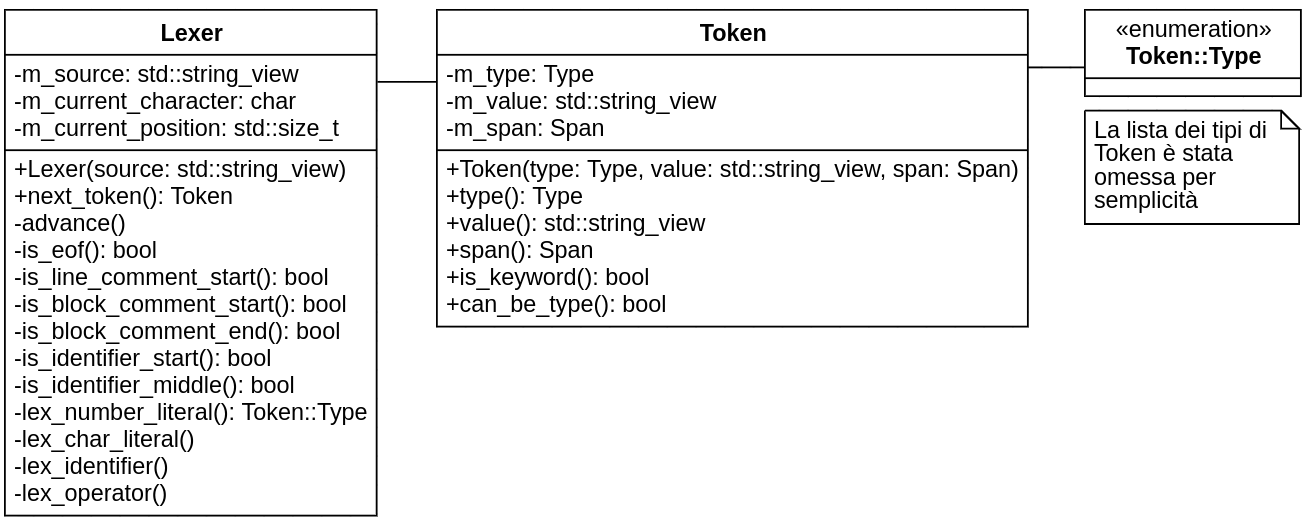
\includegraphics[width=0.9\textwidth]{figures/lexer.png}
	\caption{Diagramma UML del \texttt{Lexer}}
	\label{fig:lexer-uml}
\end{figure}

L'analisi lessicale \`e realizzata per mezzo di due classi: \texttt{Token} e \texttt{Lexer}.

La classe \texttt{Token} rappresenta i token generati dall'analisi lessicale ed \`e costituito da:
\begin{itemize}
	\item \texttt{type}: il tipo del token (un valore dell'enumerazione \texttt{Token::Type});
	\item \texttt{value}: il valore del token (una stringa);
	\item \texttt{span}: la posizione del token nel codice sorgente (un oggetto di tipo \texttt{Span}\footnote{Questo tipo di oggetto rappresenta una posizione all'interno del codice sorgente ed \`e non altro che un intervallo di due indici nella stringa contenente il sorgente del programma.}).
\end{itemize}

La classe \texttt{Lexer} realizza l'automa a stati finiti discusso nella sezione \ref{sec:analisi-lessicale} memorizzando:
\begin{itemize}
	\item \texttt{source}: il codice sorgente da analizzare (una stringa);
	\item \texttt{current\_character}: il carattere da analizzare (un carattere);
	\item \texttt{current\_position}: la posizione del prossimo carattere da analizzare (un intero).
\end{itemize}
Il metodo \texttt{advance} permette di avanzare l'automa al prossimo carattere, aggiornando \texttt{current\_character} e \texttt{current\_position} e, inoltre, di controllare se si \`e raggiunti la fine del codice sorgente. In tal caso, il metodo imposta \texttt{current\_character} al valore speciale $-1$.

Con il metodo \texttt{next\_token} \`e possibile avanzare l'automa e generare il prossimo token. Ogni volta che questo metodo viene chiamato si occuper\`a di:
\begin{itemize}
	\item rimuovere spazi vuoti e commenti;
	\item analizzare \texttt{current\_character} e generare il token corrispondente o generare un errore se il carattere non \`e valido.\footnote{Per la gestione degli errori si veda la sezione \ref{sec:gestione-degli-errori}}
\end{itemize}
In base al carattere incontrato, si delega il compito dell'analisi lessicale ad uno dei metodi presenti nel diagramma. Ad esempio, se il carattere incontrato \`e un numero si richiamer\`a il metodo \texttt{lex\_number\_literal}. Questo permette di mantenere il codice del \texttt{Lexer} pulito e facilmente estendibile, poich\'e ogni metodo si occupa di un caso specifico.

\section{\texttt{Parser}}
\label{sec:parser}

\begin{figure}[H]
	\centering
	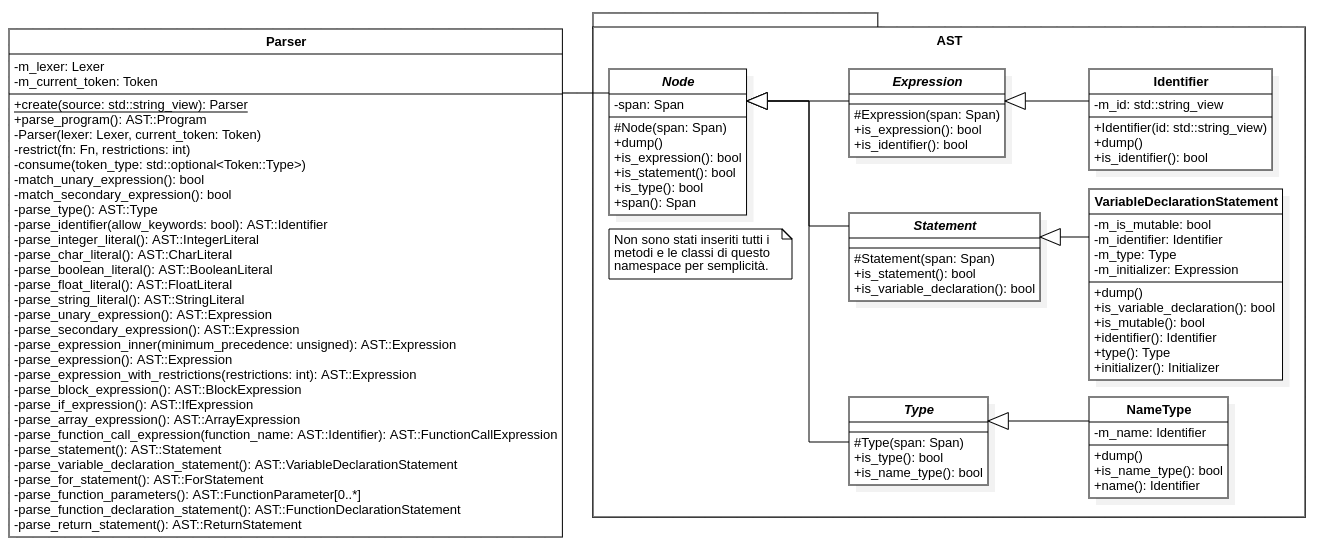
\includegraphics[width=0.9\textwidth]{figures/parser.png}
	\caption{Diagramma UML del \texttt{Parser}}
	\label{fig:parser-uml}
\end{figure}

L'analisi grammaticale \`e realizzata per mezzo della classe \texttt{Parser} e il gruppo di classi nel \textit{namespace} \texttt{AST}.

Partiamo dal descrivere il \textit{namespace} \texttt{AST}. Questo contiene la classe madre \texttt{Node} che rappresenta un generico nodo dell'AST. L'unico suo attributo \`e \texttt{span}, la posizione nel codice sorgente. Da essa derivano le seguenti classi astratte:
\begin{itemize}
	\item \texttt{Expression}: rappresenta un'espressione, ovvero un nodo che restituisce un valore;
	\item \texttt{Statement}: rappresenta uno italiano, ovvero un nodo che non restituisce un valore;
	\item \texttt{Type}: rappresenta un tipo di dato.
\end{itemize}
Da ciascuna di queste a loro volta, derivano tutte le classi che rappresentano i nodi dell'AST. Ad esempio, come \`e possibile osservare nella figura \ref{fig:parser-uml}, possiamo osservare tre nodi:
\begin{itemize}
	\item \texttt{Identifier}: sottoclasse di \texttt{Expression}, rappresenta un identificatore ed \`e descritto dall'attributo stringa \texttt{id}.
	\item \texttt{VariableDeclarationStatement}: sottoclasse di \texttt{Statement}, rappresenta una dichiarazione di variable ed \`e descritto dagli attributi:
	\begin{itemize}
		\item \texttt{is\_mutable}: un booleano che indica se la variabile \`e mutabile o meno;
		\item \texttt{identifier}: il nome della variabile (un oggetto di tipo \linebreak \texttt{Identifier});
		\item \texttt{type}: il tipo della variabile (un oggetto di tipo \texttt{Type});
		\item \texttt{initializer}: l'inizializzatore della variabile (un oggetto di tipo \texttt{Expression}).
	\end{itemize}
	\item \texttt{NameType}: sottoclasse di \texttt{Type}, rappresenta un tipo di dato descritto da un singolo identificatore, il quale sar\`a un tipo primitivo (ad esempio: \texttt{i32} o \texttt{char}).
\end{itemize}

\`E bene notare che la classe \texttt{Node} definisce una serie di metodi importanti:
\begin{itemize}
	\item il metodo \texttt{dump} che permette di stampare in formato JSON l'intera struttura del nodo; questo risulta utile in fase di debugging per verificare l'AST generato dal \texttt{Parser}.
	\item i metodi \mbox{\texttt{is\_expression}, \texttt{is\_statement} e \texttt{is\_type}} che permettono di verificare il tipo di nodo; questi metodi sono utili per effettuare controlli e conversioni di tipo durante l'analisi semantica e la generazione del codice.
\end{itemize}

Come anticipato nella sezione \ref{sec:analisi-grammaticale}, la grammatica di questo linguaggio \`e LL(1) e, citando \cite{alfred2007compilers}:
\begin{parcolumns}[colwidths={1=0.44\textwidth,2=0.44\textwidth},rulebetween=true,nofirstindent=true,sloppy=true]{2}
	% LTeX: language=en_us
	\colchunk{
		\leftskip=1em
		``The first ``L'' in LL(1) stands for scanning the input from left to right, the second ``L'' for producing a leftmost derivation, and the ``1'' for using one input symbol of \emph{lookahead} at each step to make parsing action decisions.''
	}
	% LTeX: language=it
	\colchunk{
		\leftskip=1em
		``La prima ``L'' in LL(1) indica che si analizza l'input da sinistra verso destra, la seconda ``L'' indica che si produce una derivazione sinistra e l'``1'' per usare un \emph{lookahead} di un simbolo d'input a ogni passo per fare decisioni di analisi grammaticale.''
	}
	\colplacechunks
\end{parcolumns}

I parser costruiti per questo tipo di grammatica, e di conseguenza quella di BugginOut, sono detti \emph{predictive}, ovvero dei parser \emph{recursive descent} senza il bisogno di \emph{backtracking}. I parser \emph{recursive descent} sono dei particolari parser \emph{top-down} costruiti con delle procedure ricorsive dove ognuna di queste riflette un non-terminale della grammatica. Si \`e scelto di costruire il parser seguendo questo approccio proprio perch\'e il codice che ne risulta \`e molto semplice, leggibile ed efficiente, non essendo richiesto il backtracking. Di fatti, gli unici due attributi richiesti per mantenere lo stato del parser sono:
\begin{itemize}
	\item \texttt{lexer}: il \texttt{Lexer} che fornisce i token da analizzare;
	\item \texttt{current\_token}: il token corrente da analizzare.
\end{itemize}

Ogni metodo del parser, che rappresenta un non-terminale della grammatica, analizzer\`a il token corrente e, se corretto, lo \emph{consumer\`a}. Questa operazione viene implementata dal metodo \texttt{consume} e corrisponde ad ottenere il prossimo token dal \texttt{Lexer} e aggiornare \texttt{current\_token}. Il metodo prevede un parametro opzionale che permette di specificare il tipo di token atteso. Se il token corrente non corrisponde al tipo atteso, viene generato un errore di sintassi. Se il tipo di token non viene specificato, il metodo consuma il token corrente.

\`E importante notare che per realizzare dei \emph{predictive parser} la grammatica deve soddisfare due requisiti molto importanti:
\begin{itemize}
	\item non deve contenere ricorsioni sinistre;
	\item non deve essere ambigua.
\end{itemize}

La grammatica, per come \`e stata definita, non contiene ricorsioni sinistre ma \`e ambigua nella gestione delle espressioni e dei loro operatori. Questo \`e stato fatto volutamente per due ragioni:
\begin{itemize}
	\item \`e possibile cambiare la precedenza ed associativit\`a degli operatori in modo semplice, senza dover modificare la grammatica;
	\item il parser non spende tempo utile nell'analizzare produzioni \textit{singole} ovvero costituite da un solo non-terminale.
\end{itemize}
In ogni caso, l'amgiguit\`a deve essere gestita e, per farlo, si utilizza un algoritmo di \emph{precedence climbing}.

Introdotto per la prima volta da \cite{barron1981bcpl}, l'idea alla base \`e quella di avere una funzione ricevere in input un'espressione e una \emph{precedenza minima}. Durante l'analisi, la funzione consuma gli operandi fino a quando incontra operatori la cui precedenza \`e maggiore o uguale a quella minima. Se un operatore ha precedenza inferiore, l'espressione si interrompe e si ritorna al livello di ricorsione precedente. L'associativit\`a di un operatore viene gestita in maniera molto elegante, con un semplice controllo effettuato prima della prossima chiamata ricorsiva: se l'operatore \`e associativo a sinistra allora ne aumenta di un'unit\`a la precedenza, altrimenti la lascia invariata. Per capire meglio come funziona, vediamo degli esempi:
\begin{itemize}
	\item Si supponga di voler analizzare l'espressione \texttt{a + b + c}, che la precedenza di \texttt{+} sia 2 e che \texttt{+} sia associativo a sinistra.

	La prima chiamata ricorsiva consuma \texttt{a} e chiama la funzione con precedenza minima $2 + 1$ essendo \texttt{+} associativo a sinistra. La prossima chiamata trover\`a nuovamente \texttt{+} con precedenza $2$ minore della precedenza minima $2 + 1$. Allora esce e l'espressione generata sar\`a \linebreak \texttt{(a + b) + c}.
	\item Adesso si supponga di essere nelle stesse condizioni dell'esempio precedente con l'unica differenza che \texttt{+} sia associativo a destra.

	Durante l'analisi la seconda chiamata alla funzione avr\`a precedenza minima $2$ e, dunque, quando incontrer\`a \texttt{+} lo consumer\`a e l'espressione generata sar\`a \texttt{a + (b + c)}.
\end{itemize}

Questo algoritmo \`e implementato tramite tre funzioni:
\begin{itemize}
	\item \texttt{parse\_expression\_inner}: \`e la funzione ricorsiva di cui si \`e discusso fino ad ora;
	\item \texttt{parse\_primary\_expression}: \`e la funzione che analizza il non-terminale \texttt{<primary>};
	\item \texttt{parse\_secondary\_expression}: \`e la funzione che, prese la parte sinistra e l'operatore di un'espressione ottenuti da \linebreak \texttt{parse\_expression\_inner}, analizza la parte destra (se necessario) e li combina per ottenere l'espressione intermedia.
\end{itemize}
Per gestire la precedenza e l'associativit\`a degli operatori si usa una classe ausiliaria detta \texttt{OperatorData} che mantiene questi due valori per ognuno degli operatori. Per rappresentare la precedenza si usa un intero senza segno che, se basso indica una bassa precedenza, se alto indica una alta precedenza. Per l'associativit\`a si usa una semplice enumerazione di due valori: \texttt{Left} se a sinistra e \texttt{Right} se a destra.

\section{\texttt{Typechecker}}
\label{sec:typechecker}

\section{\texttt{Transpiler}}
\label{sec:transpiler}

\section{Gestione degli errori}
\label{sec:gestione-degli-errori}
